\chapter{基于传统视觉算法的无人机目标跟踪方法研究}

针对目标检测问题,很多学者提出了不同的解决方法,但目标实时监测问题中的所涉及的目标尺度变化、被遮挡和实时性等问题仍然没有得到有效解决。本章针对无人机自主降落过程中的目标跟踪问题进行进一步分析,并提出了满足实时性需求的目标跟踪算法。

\section{目标跟踪问题的概述}
One-shot Tracking问题的核心是目标位置的先验信息唯一,一般定义为图像序列第一帧$I_1$的位置信息$b_1$(Bounding Box),且该问题针对单一目标图像进行跟踪。这一概念于2006年由华人研究者李飞飞提出\cite{fei2006one},并有CMT算法\cite{Nebehay2016}的作者Georg Nebehay将这一概念引入到目标跟踪领域。在算法的运行过程中,随着图像目标的连续运动,跟踪算法可以利用之前的图像纹理信息和位置信息作为新的先验信息对当前图像进行解算,其基本流程如算法\ref{al:one_shot_tracking}所示。

传统的实时跟踪方法的主要工作是在线对模型进行计算和更新,算法在运行过程中,基本不涉及和使用离线运算结果。这些跟踪算子(Tracker)主要通过数学公式来完成对跟踪目标特征的描述,这种数学公式对模型描述能力的好坏决定着整体算法性能的优劣。同时,由于传统方法的跟踪算子无法重复利用大量现有数据,其算法性能无法随着数据量的增加而得到持续性改善。这种方法适用于典型目标的跟踪,例如行人跟踪和人脸跟踪等。

\begin{algorithm2e}[H]
	\SetAlgoLined
%	\KwData{this text}
%	\KwResult{how to write algorithm with \LaTeX2e }
	\BlankLine
	\SetKwInOut{Input}{Input}
	\SetKwFunction{Track}{Track}
	\SetKwFunction{Update}{Update}
	\SetKwFunction{Initialization}{Initialization}
	\Input{Image sequence $I_1, ..., I_T$ with bounding box $b_1$}
	\Initialization($I_1$, $b_1$)\;
	\For{$i=2$ \KwTo $T$}{
		$b_i\ \leftarrow$ \Track{$I_i$}\;
		$b_i\ \leftarrow$ \Update($b_t$, $b_{t-1}$, ..., $b_1$) \;
	}
	\caption{One-shot Tracking 算法框架}
	\label{al:one_shot_tracking}
\end{algorithm2e}
综上所述,本文涉及到的无人机降落过程中的跟踪问题划归为One-shot Tracking问题。在后续使用的目标跟踪数据集中,无人机第一帧所在的中心位置和矩形框通过手动标记共处,后续图像序列根据第一帧给出的信息进行进一步的迭代和解算。

\section{形态学滤波方法进行图像预处理}

形态学滤波(Morphological Filtering)方法是一组非线性图像运算算子。该系列算子主要包括腐蚀(Erode)、膨胀(Dilate)、开运算(Opening)和闭运算(Closing)四种基本运算。在此四种运算的基础之上,一般还可以拓展出边缘提取、凸包运算、连通区域标记等复杂运算。通常而言,由于上述算子主要通过像素之间位置,形态学处理的对象为二值图像。

在有人机的感知规避领域,机载雷达是应用最为广泛的周边环境的感知器。除此之外,安装在机身各个位置的摄像头也是感知飞行器周边环境的重要传感器。一般而言,这些摄像头主要用于在空中识别周边的其他飞行器。由于民航飞行器的空间间隔一般较大,飞行器的成像尺寸一般较小,传统的预处理方法容易将这类小型目标当做噪声忽略。2011年,卡内基梅隆大学的三位学者使用形态学滤波方法对微小无人机检测的图像进行预处理\cite{dey2011cascaded},这篇文章图像预处理和图像检测的研究背景与本文的背景类似。
\begin{figure}[ht]   
	\centering
	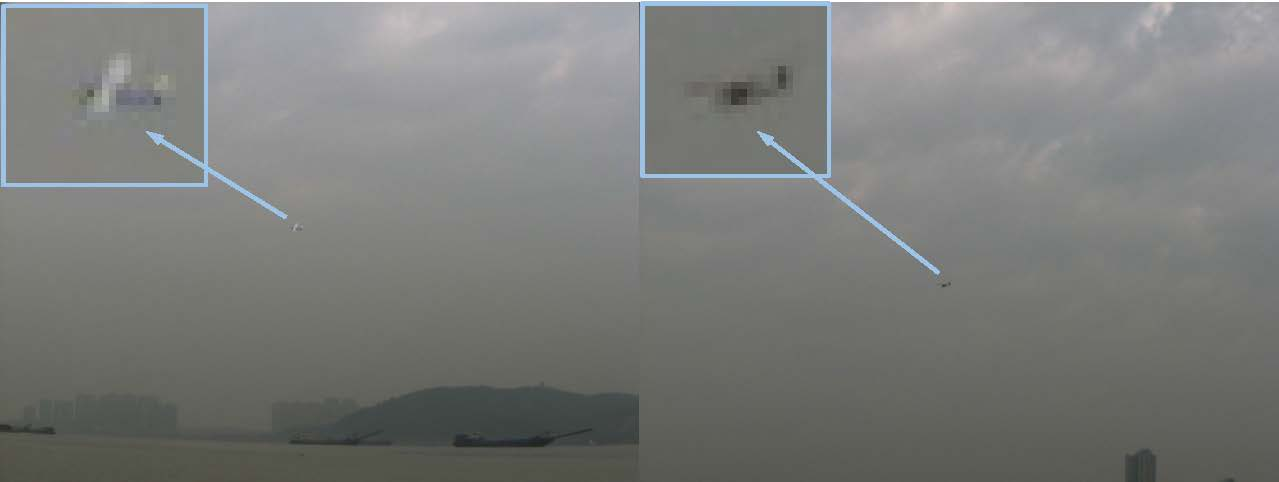
\includegraphics[width=\textwidth]{figs/chp03/01_small_uav_light_black.pdf}
	\caption{小型无人机$400\ m$在可见光相机成像效果}
	\label{fig:01_small_uav_light_black}
\end{figure}

针对本文涉及到的无人机目标识别问题,形态学滤波对图像预处理仍然是一种较为理想的方法。无人机距离摄像机较远的位置,由于机翼颜色和光照的影响,无人机的成像一般为一个亮点或一个暗点。对于试验中使用的白色无人机而言,在一次降落过程中,该无人机在距离摄像机$400\ m$左右的距离时,其成像效果如图\ref{fig:01_small_uav_light_black}所示。图中左上侧的矩形框是无人机目标放大后的结果。通过成像结果可以看到,左侧图像为无人机在转弯时,由于机翼为白色且面积较大,因此成像为一个白色为主的亮斑;右侧图像是无人机转弯完成后,无人机侧面虽然仍为白色,但由于反光面积相对较小,所以在相机中的成像为黑色为主的亮斑。


对于试验中使用的中等型号的无人机而言,其在距离摄像机$800\ m$左右的距离时,其成像效果如图\ref{fig:02_big_uav_light_black}所示。通过比较两种型号无人机的成像特性,本文设计将开运算与闭运算处理结果相减作为预处理的结果,主要针对小型无人机出现的白色和黑色亮斑变化情况进行处理。

\begin{figure}[ht]   
	\centering
	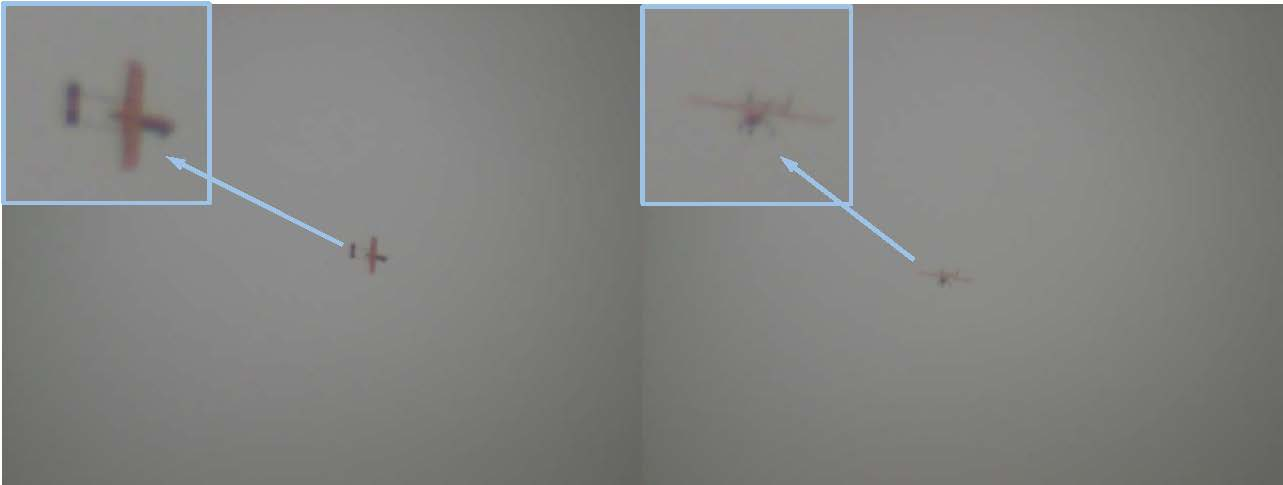
\includegraphics[width=\textwidth]{figs/chp03/02_big_uav_light_black.pdf}
	\caption{中型无人机$800\ m$在可见光相机成像效果}
	\label{fig:02_big_uav_light_black}
\end{figure}

开运算的特点是先进行腐蚀运算,再进行膨胀运算,能够消除细小物体,突出物体边缘,即亮出的区域增大。闭运算的特点是先进行膨胀运算,再进行腐蚀运算,能够消除细小空洞,使得临近的物体相互连通,即暗处的区域增大。为了利用开运算和闭运算结果的优点,该滤波方法的基本框架如图\ref{fig:04_morphogolical_method}所示。在Ubuntu环境下使用Python实现上述预处理算法,开运算和闭运算分别对每一帧图像($640 \times 480$)进行处理时间为$0.009\ s$至$0.013\ s$,整体时间消耗约为$0.016\ s$。在后续目标跟踪过程中,矩形框区域的像素面积远小于完整图像面积,因此该算法能够满足系统的实时性需求。

\begin{figure}[ht]   
	\centering
	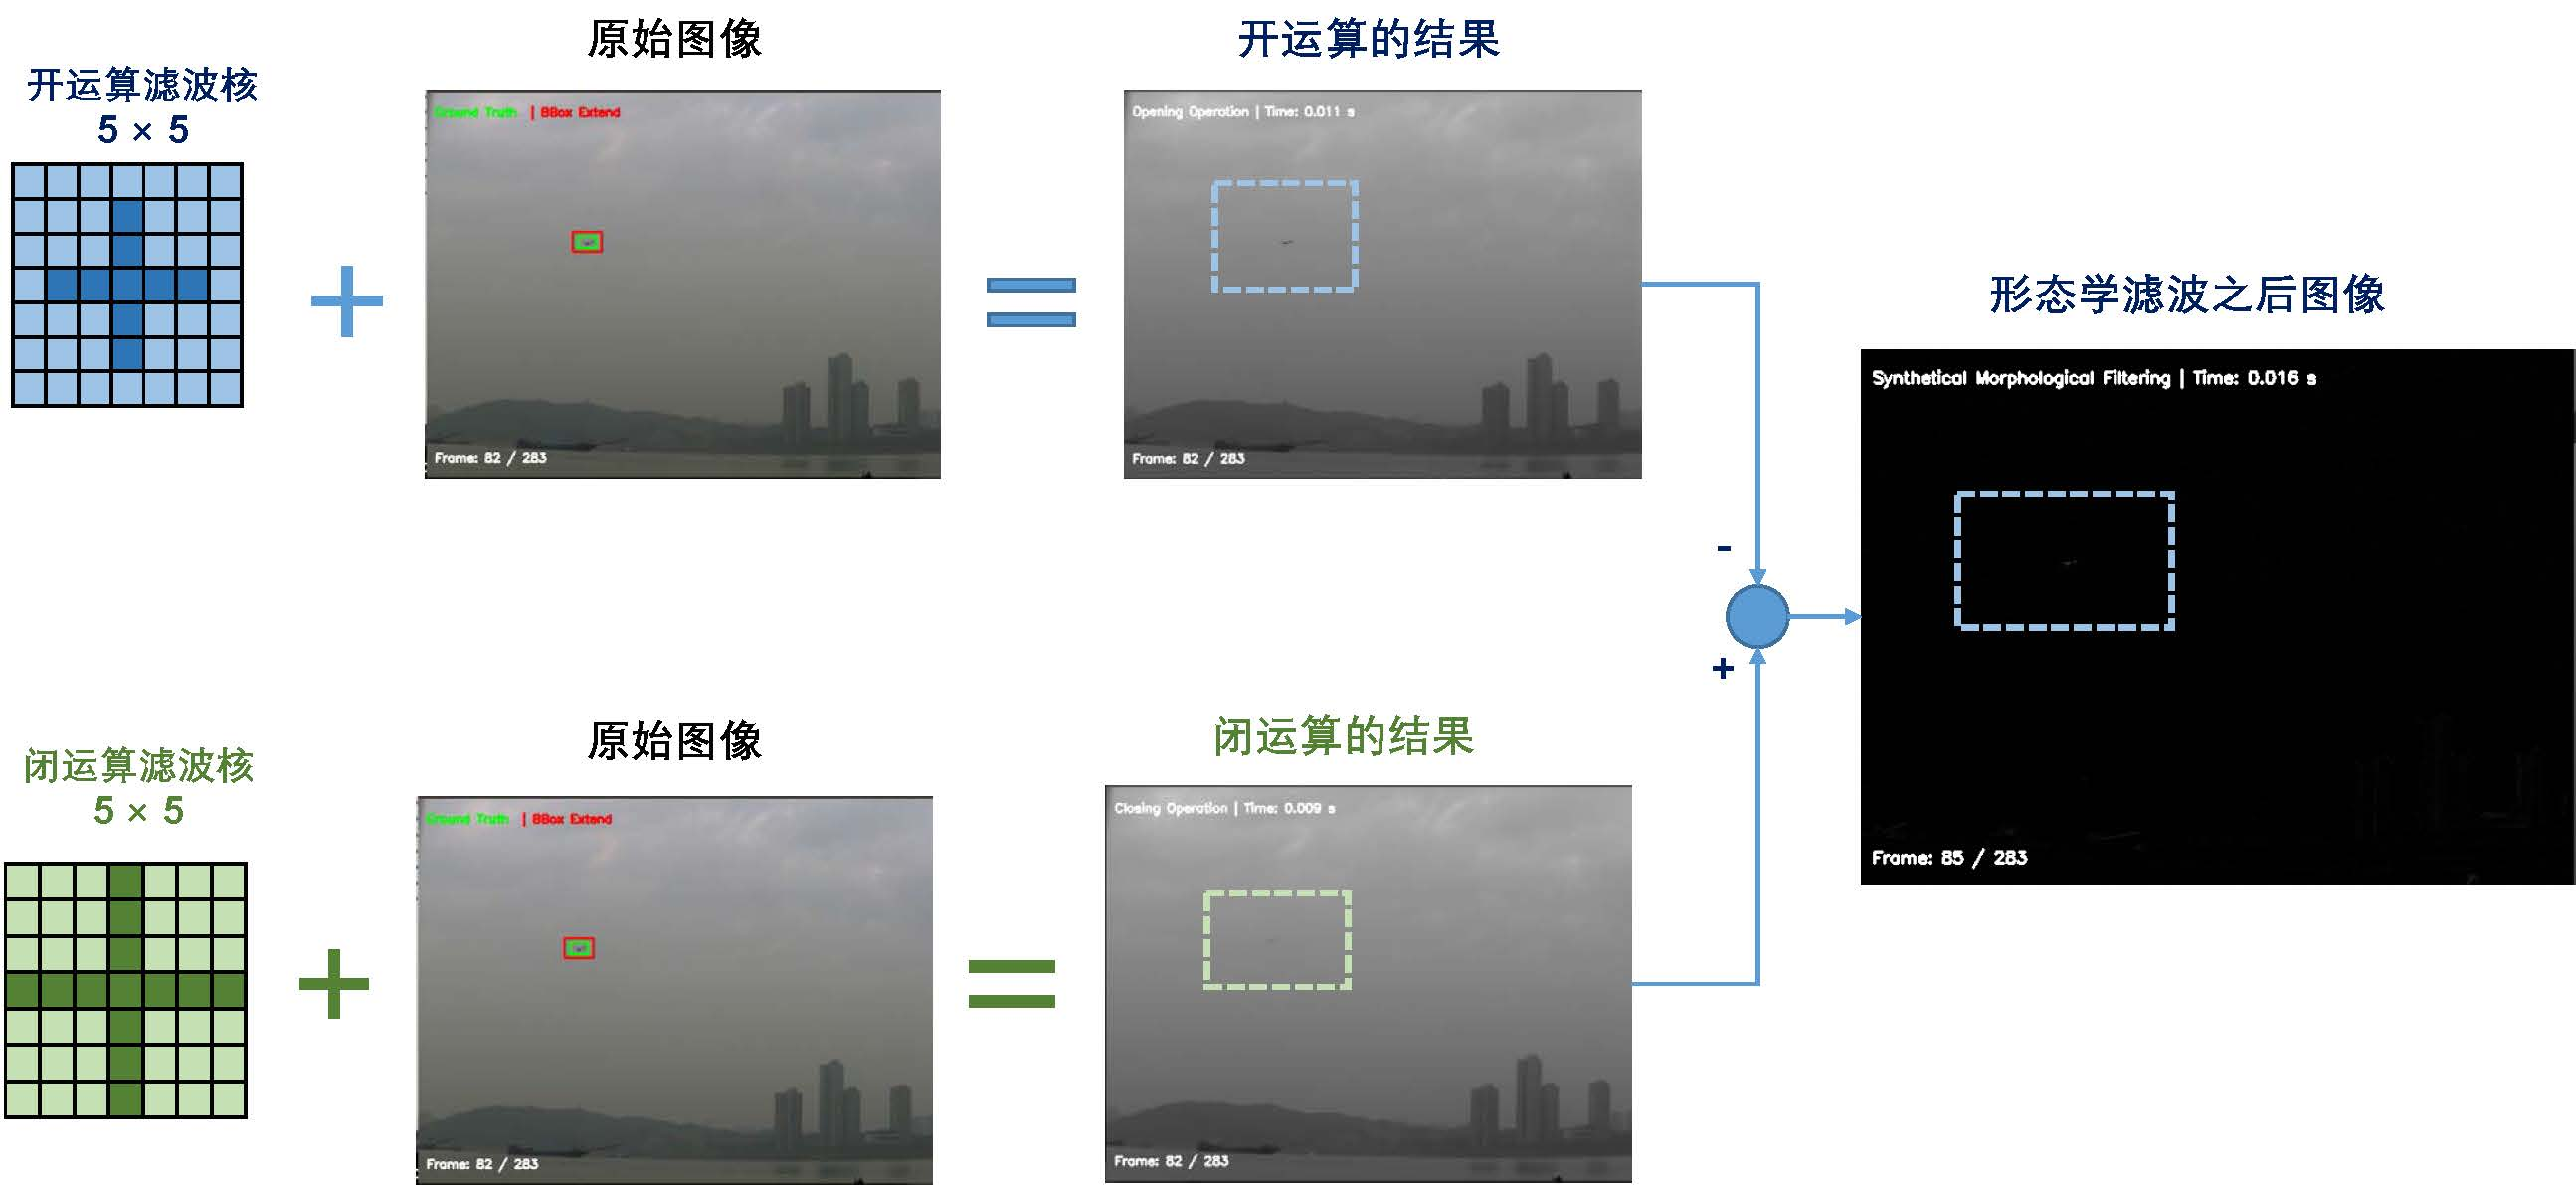
\includegraphics[width=\textwidth]{figs/chp03/04_morphogolical_method.pdf}
	\caption{形态学滤波预处理框架}
	\label{fig:04_morphogolical_method}
\end{figure}

将该算法运用到图\ref{fig:01_small_uav_light_black}中所示的图像,预处理之后的结果如图\ref{fig:03_small_uav_with_morphological}所示。结果表明,闭运算的结果减去开运算的结果能够将暗处和亮出的区域均进行筛选和保留,进一步突出小型无人机在远端时的图像特征,为后续的目标跟踪问题打下良好基础。

\begin{figure}[ht]   
	\centering
	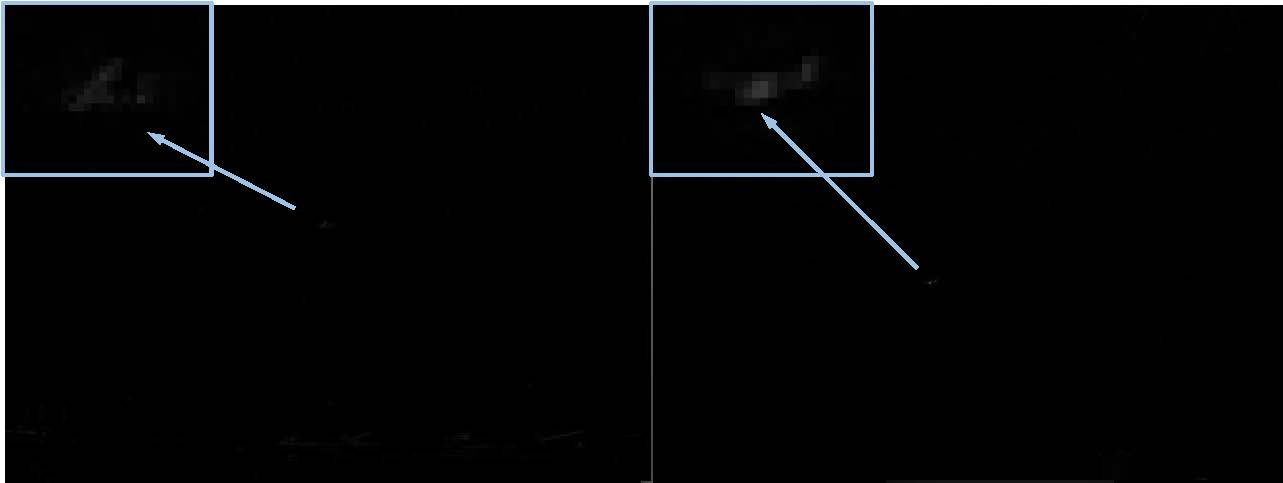
\includegraphics[width=\textwidth]{figs/chp03/03_small_uav_with_morphological.pdf}
	\caption{小型无人机在两种状态下使用形态学滤波处理之后的结果}
	\label{fig:03_small_uav_with_morphological}
\end{figure}


%\section{基于角点检测的目标跟踪方法研究}


\section{基于Tracking-Learning-Detection框架的目标跟踪研究}
\subsection{Tracking-Learning-Detection基本框架}
One-shot跟踪问题的核心就是如何随着图像序列的信息增加,合理有效的使用目标自身包含的表观信息(Apperance)和目标周边的环境信息。1979年Box提出一个对于模型鲁棒性的观点\cite{box1979robustness}:

\begin{center}
All models are wrong, but some are useful.
\end{center} 



上述对模型描述的观点来自统计学思想,该思想给出了解决One-shot Tracking问题中对序列图像信息处理的一种宏观思路:系统如何在接受新信息的同时,对旧信息进行合理的平衡,以此保持模型的鲁棒性,却不失对模型实时变化的描述。TLD(Tracking-Learning-Detection)\cite{kalal2012tracking}框架是一种针对One-shot Tracking问题的提出的一种长时间跟踪(Long-term Tracking)算法框架。该算法对连续的的图像序列中的唯一目标进行不间断跟踪,无论该物体是否暂时离开画面,或者被遮挡和发生形变,都不会影响跟踪效果。该算法框架包含以下三个部分:
\begin{compactenum}
	\item 跟踪器(Tracker),通过连续帧图像来预估所追踪对象的运动,这里假设帧与帧之间目标的相对运动有限,并且追踪目标保持在图像中始终可见。追踪器可能会出现追踪失败的情形,并且在目标跳出相机视野后无法恢复追踪。
	\item 检测器(Detector),将各帧图像视为独立,并对每一帧图像都进行全扫面,以找出图像中所有与目标外貌相似的候选样本。该探测器会产生两类错误:错误的正样本(False Positives)和错误的负样本(False Negatives)。
	\item 学习(Learning),学习过程实时观测追踪器和探测器的执行,并预估探测器的错误,生成训练样例以使能在未来避免类似的错误。学习组件假设追踪器和探测器都有可能出现失败执行,但学习组件的引入可以使得探测器生成更多的追踪目标外观,以区别背景。
\end{compactenum}

该算法的整体工作示意图,如图\ref{fig:02_big_uav_light_black}所示\cite{kalal2012tracking}。通过该示意图可以看到,跟踪、学习和检测三个主要环节在算法运行过程中各自独立运行且直接存在数据交互,这种对新信息和历史信息的处理方式,能够保证对目标跟踪的稳定性,同时也满足系统的实时性需求。

\begin{figure}[ht]   
	\centering
	\includegraphics[width=0.4\textwidth]{figs/chp04/chp04_20_TLD_framework.pdf}
	\caption{Tracking-Learning-Detection跟踪框架}
	\label{fig:chp04_20_TLD_framework}
\end{figure}


\subsection{跟踪器的设计}
TLD的作者提出:一个好的跟踪算法应当具备正反向连续性(Forward-backward Consistency)\cite{kalal2010forward},即图像序列是正时序进入系统还是反时序进入系统,系统对目标跟踪之后所产生的轨迹应当是相同的。根据该特性,作者定义了跟踪器的向前向后误差(Forward-backward Error, FB):当前$t$时刻的初始位置为$\mathbf{p}(t)$,基于该位置得到$t+1$时刻的目标位置$\mathbf{p}(t+1)$,再根据得到的$\mathbf{p}(t+1)$位置反向计算$t$时刻的位置$\epsilon = \mathbf{p}'(t)$,定义$||\mathbf{p}(t)-\mathbf{p}'(t)||$作为向前向后误差的度量。

该误差的直观表达如图\ref{fig:chp04_21_FB_Error}所示。该图像是将无人机降落过程中的连续两帧图像叠加起来显示在一幅图像中。其中红色无人机表示$t$时刻无人机成像位置,蓝色无人机表示$t+1$时刻无人机成像位置。在前向计算过程中,红色点1在对应得到蓝色点,该蓝色点在反向运算中正确得到红色点1,此时的前向后向传递误差为零。但图中红色点2在前向计算过程中得到的对应蓝色点并没有在反向运算中返回到正确位置,而是反向对应得到红色点3,此时的前向后向传递误差需要通过上述定义进行求解。为更快的计算连续两帧的对应点位置,主要采取Lucas-Kande Model\cite{lucas1981iterative}来完成图h像中兴趣点的跟踪,该方法也是经典光流算法中使用的模型,使用$\mathbb{LK}$定义为该模型算子的数学记号。则上述坐标点直接的关系定义为
\begin{align}
&\mathbf{p(t+1)} = \mathbb{LK}(\mathbf{p(t)}) \\
&\mathbf{p(t)}' = \mathbb{LK}(\mathbb{LK}(\mathbf{p(t)}))
\end{align}
通过定义前向传递误差的阈值$\theta_{FB}$,对多个兴趣点的$\epsilon$进行筛选,留下误差相对较小的兴趣点。

同时,对于相同的兴趣点,还需要对该点周边的图像区域进行描述和评估,这种描述一般定义为归一化互相关(Normalized Cross Correlation, NCC)值。定义两个不同兴趣点的周边图像区域为$P_1$和$P_2$,则NCC的数学表达为
\begin{equation}
NCC(P_1, P_2) = \frac{1}{n-1}\sum_{x=1}^{n}\frac{(P_1-\mu_1)(P_2-\mu_2)}{\sigma_1\sigma_2}
\end{equation}
其中$\mu_1$、$\mu_2$、$\sigma_1$和$\sigma_2$分别是图像区域$P_1$和$P_2$的所有像素的均值和方差。文献\cite{lewis1995fast}证明基于NCC的相似度计算方法对光照变化不敏感。

\begin{figure}[ht]   
	\centering
	\includegraphics[width=0.8\textwidth]{figs/chp04/chp04_21_FB_Error.pdf}
	\caption{Forward-backward Error示意图}
	\label{fig:chp04_21_FB_Error}
\end{figure}

在使用上述两种方法得到兴趣点的FB和NCC数值之后,一般采用中值滤波(Median Filter)的方法分别计算出两种度量量的中值$\text{med}_{FB}$和$\text{med}_{NCC}$之后,对兴趣点进一步筛选,进而得到对下一帧矩形框$b(t+1)$的参考点。跟踪算法的伪代码如算法\ref{alg:tld_tracking}所示。

\begin{algorithm2e}[ht]
	\SetAlgoLined
	%	\KwData{this text}
	%	\KwResult{how to write algorithm with \LaTeX2e }
	\BlankLine
	\SetKwInOut{Input}{Input}
	\SetKwFunction{TLD}{TLD}
	\SetKwFunction{MedianFlow}{MedianFlow}
	\SetKwFunction{Transform}{Transform}
	\Input{Image $I(t)$,Bounding Box $b(t)$}
	$\{\mathbf{p}(t)_1, \mathbf{p}(t)_2,...,\mathbf{p}(t)_n\}$ $\leftarrow$ \Initialization($b_I$)\;	
	\For{$\mathbf{p}(t)_i$}{
		$\mathbf{p}(t+1)_i\leftarrow \mathbb{LK}(\mathbf{p}(t)_i)$\;
		$\mathbf{p}(t)'_i\leftarrow \mathbb{LK}(\mathbf{p}(t+1)_i)$\;
		$\epsilon_i \leftarrow ||\mathbf{p}(t)'_i-\mathbf{p}(t)_i||$ \;
		$\eta_i \leftarrow NCC(P_1, P_2)$ \;
	}
	$\text{med}_{FB} \leftarrow$\MedianFlow($\{\epsilon_i\}$) \;
	$\text{med}_{NCC} \leftarrow$\MedianFlow($\{\eta_i\}$) \;
	$\{\bar{\mathbf{p}}_i\} \leftarrow  \{\mathbf{p}(t)_i,\mathbf{p}(t)'_i|\text{med}_{FB} \le \epsilon_i, \text{med}_{NCC} \ge \eta_i \}$\;
	$b(t+1) \leftarrow$\Transform($b(t),\{\bar{\mathbf{p}}_i\}$)\;
	\caption{TLD框架中的Tracking算法}
	\label{alg:tld_tracking}
\end{algorithm2e}


\subsection{检测器的设计}
在上述跟踪器的设计主要在兴趣点周边对图像进行跟踪,但考虑到目标跟踪有可能存在持续偏移或者目标被瞬间遮盖,因此需要设计检测器来减少目标跟踪丢失的情况。与跟踪器的设计思路不同,检测器并不使用连续两帧图像中的信息进行识别,而是将各帧图像视为相互独立的信息。检测器通过对每一帧图像进行全局搜索,以找出图像中所有与目标表观特征相似的候选样本。此外,检测器的另一个重要作用是通过对候选样本筛选,来更新学习器。这里需要注意,通过对图\ref{fig:02_big_uav_light_black}观察可以发现,与跟踪器和学习器不同,检测模块有两个信息输出流,其中一个是将检测好的目标传递给跟踪器,另一个是将检测过程中的正负样本信息传递给学习器。

%一般而言,探测器会产生两类样本:错误的正样本(False Positives)和错误的负样本(False Negatives)。
检测器的检测范围是当前帧的完整图像,但由于对当前帧目标的尺寸信息没有先验知识,因此需要设计密度足够大、尺寸种类足够多的扫描窗网格(Grid)来对全图进行扫描。一般通过可能出现的比例(Scales)和平移(Shifts)的初两个参数进行构建。例如,定义比例值$s=1.2$,水平和竖直方向的尺度变化$a=10$,最小边界框大小为20个像素。针对一个尺寸为$640\times480$的图像,大约需要生成约$5\times10^4$个扫描窗口。由于对于每一个扫描窗口的检测是相对独立的,因此在程序编写的过程中,可以将上述窗口的检测通过线程设计来提高检测速度。

针对每一个检测窗口,主要设计一个级联分类器(Cascaded Classifier),该级联分类器由三个算法不同的分类器串行组成。这三种算法分别是表观特征筛选(Patch Variance)、组合分类器(Ensemble Classifier)和最近邻筛选(Nearest Neighbor)。在每一个分类阶段,上述扫描窗口被一一筛选,最终留下可信度较高的区域。
\begin{figure}[ht]   
	\centering
	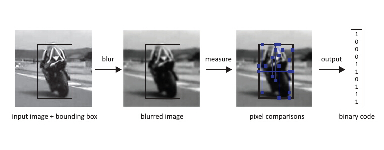
\includegraphics[width=\textwidth]{figs/161002_Thesis_Tracking_Section_04.pdf}
	\caption{集成分类器示意图}
	\label{fig:161002_Thesis_Tracking_Section_04}
\end{figure}

%正样本区域的放射变换对每个正样本区域,进行$±1\%$范围的偏移,$±1\%$范围的尺度变化,$±10\%$范围的平面内旋转,并且在每个像素上增加方差为5的高斯噪声(确切的大小是在指定的范围内随机选择的),那么每个box都进行20次这种几何变换,那么10个box将产生200个仿射变换的bounding box,作为正样本。

Patch Variance: 首先利用积分图求出当前要分类扫描窗的灰度值期望,再根据期望计算出方差,与原bounding-box的方差作对比,方差小于bounding-box方差的$50\%$的扫描窗都不会通过这个分类器。(这里的阈值是可以调整的)

集成分类器(Ensemble Classifier) 主要采用随机森林(Random Forest )的方法,其中特征选择2bitBP和Pixel Comparisions特征。Pixel Comparisons 的实现方法如下:首先,图像与高斯核进行方差为3像素的卷积,以提高转换稳健性和图像噪声。然后,根据决策树方法进行比较。


Random Forest 方法 :andom Forests方法主要源于BinaryDecision Trees。传统的决策树主要由一系列子二叉树组成,在每一个节点通过简单的YES/NO问题进行分类。在叶子节点,表明数据所属的类型。因此,对于一个决策树而言,一组特征数据通过不同节点的判断,最终得到一个分类结果。通过训练,我们可以根据训练数据的特征,构建一棵“完美”的决策树用于实际应用。但一般而言,单棵决策树训练速度较快,可以快速处理大量数据,但存在过拟合现象,在实际应用中误差较大。为解决单棵决策树存在的缺陷,1995年Ho以及2001年Breiman分别提出采用多个决策树并引入随机特征方法,即Random Forests。其中,通过构建相互独立的多个决策树,从而提高数据处理的多样性;通过在学习过程中引入随机性,来增强系统的鲁棒性。最后,根据少数服从多数的投票原则,判定一个数据的类别。

对样本的处理。Bootstrap Sampling 思想。通过有重复的随机抽取样本,重新组成新的样本集。原始数据集的数学表示如下:
$$\mathbf{\{Dat}{{\mathbf{a}}_{\mathbf{1}}}\mathbf{,Dat}{{\mathbf{a}}_{\mathbf{2}}}\mathbf{,Dat}{{\mathbf{a}}_{\mathbf{3}}}\mathbf{,Dat}{{\mathbf{a}}_{\mathbf{4}}}\mathbf{,Dat}{{\mathbf{a}}_{\mathbf{5}}}\mathbf{,Dat}{{\mathbf{a}}_{\mathbf{6}}}\mathbf{,Dat}{{\mathbf{a}}_{\mathbf{7}}}\mathbf{,Dat}{{\mathbf{a}}_{\mathbf{8}}}\mathbf{,Dat}{{\mathbf{a}}_{\mathbf{9}}}\mathbf{,Dat}{{\mathbf{a}}_{\mathbf{10}}}\mathbf{\}}$$

随机抽取之后的数据集如下:
$$\mathbf{\{Dat}{{\mathbf{a}}_{\mathbf{7}}}\mathbf{,Dat}{{\mathbf{a}}_{\mathbf{6}}}\mathbf{,Dat}{{\mathbf{a}}_{\mathbf{3}}}\mathbf{,Dat}{{\mathbf{a}}_{\mathbf{1}}}\mathbf{,Dat}{{\mathbf{a}}_{\mathbf{1}}}\mathbf{,Dat}{{\mathbf{a}}_{\mathbf{8}}}\mathbf{,Dat}{{\mathbf{a}}_{\mathbf{7}}}\mathbf{,Dat}{{\mathbf{a}}_{\mathbf{2}}}\mathbf{,Dat}{{\mathbf{a}}_{\mathbf{9}}}\mathbf{,Dat}{{\mathbf{a}}_{\mathbf{5}}}\mathbf{\}}$$

可以看到,则随机抽取之后的数据样本集中,不仅样本集的顺序发生了改变,个别样本集也出现了重复。

子特征集的提取。系统不再对全部特征进行训练,而是从中随机选出一个子集进行训练,基于这些子集得到不同类型的决策树。


Random Fern 方法:Random Fern 的思想就是用多个特征组合来表达对象。


\begin{figure}[ht]   
	\centering
	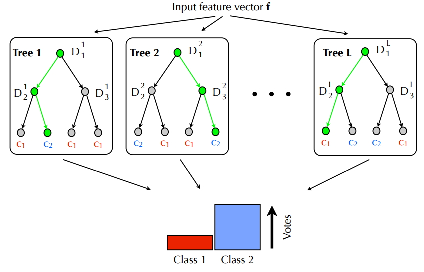
\includegraphics[width=\textwidth]{figs/161002_Thesis_Tracking_Section_05.pdf}
	\caption{集成分类器示意图}
	\label{fig:161002_Thesis_Tracking_Section_05}
\end{figure}

Random Fern 方法基于贝叶斯理论,主要是对简单贝叶斯分类器(Navie Bayes Classifiers)的改进。对于不同的特征$(f_1, f_2, ..., f_N)$而言,分类的最大化这些特征的后验概率:

$$\arg \max_{k}P(C_k|f_1, f_2, ..., f_N)$$

通过贝叶斯公式可以转换为求解最大化极大似然函数与先验概率的乘积

$$\arg \max_{k}P(f_1, f_2, ..., f_N|C_k)P(C_k)$$

这里引入各个特征相互独立的基本假设,方程可以将极大似然函数的求解进一步化简为
$$
P(f_1, f_2, ..., f_N|C_k)=\prod\limits_{i=1}^{N}P(f_i|C_k)
$$
此时,可以得到新的分类公式
$$
\arg\max_kP(C_k)\prod\limits_{i=1}^{N}P(f_i|C_k)
$$
但是在实际问题的求解过程中,每个特征的独立性假设过于严格,因此2007年的CVPR M.Oezuysal中提出Semi-Navie Bayes方法,即将特征进行分组,认为组与组之间保持严格的独立性,而组件的特征相互依赖。假设所有的特征可以分为$L$个组别,每个组别中包含$S$个特征,每个组别被称为Ferns,每一个特征组的表达为
$$
\mathbf{F}_l=\{f_{l,1}, f_{l,2},..., f_{l,S}\}
$$
为了在检测过程中计算便捷,选用二维编码的方式对图像进行描述,因此每一个特征满足$f_n\in\{{0,1}\}$。由此,可以进一步将极大似然函数重新表达
$$
P(f_1, f_2, ..., f_N|C_k)=\prod\limits_{i=1}^{L}P(\mathbf{F}_l|C_k)
$$
基于特征分组的分类公示为
$$
\arg\max_kP(C_k)\prod\limits_{i=1}^{L}P(\mathbf{F}_i|C_k)
$$
在实际训练过程中,由于训练样本数量较少,会导致分类概率为零的情况。因此,我们认为$P(\mathbf{F}|C_k)$符合Dirchlet分布,因此设定一个最小的概率输出
$$
p(\mathbf{F}=z|C_k)=\frac{\mathbb{N}(\mathbf{F}=z|C_k)+1}{\sum_{z=0}^{2^S-1}(\mathbb{N}(\mathbf{F}=z|C_k)+1)}
$$
其中,$\mathbb{N}(\mathbf{F}=z|C_k)$是计算在类别$C_k$情况下,观测到$\mathbf{F}=z$的特征个数。

\subsection{学习器的设计}
学习模块(Leaner)学习过程实时观测追踪器和探测器的执行,并预估探测器的错误,生成训练样例以使能在未来避免类似的错误。学习组件假设追踪器和探测器都有可能出现失败执行,但学习组件的引入可以使得探测器生成更多的追踪目标外观(generalizes to more object appearances),以区别背景。

PN学习即PN learning, P指代Positive Constraint,也称之为P-expert或者growing event,N指代Negative Constraint,也称之为N-expert或者pruning event。

P-expert的作用是发现目标的新的外观(形变),并以此来增加正样本的数量,从而使得检测模块更具鲁棒性;N-expert的作用是生成负的训练样本。N-expert的前提假设是,(被跟踪的)前景目标仅可能出现在视频帧中的一个位置,因此,如果前景目标的位置是确定的,那么其周围必然是负样例。

TLD模块中的PN学习作用是通过对视频序列的在线处理来逐步改善检测模块(TLD中的Detection)的性能。对视频中的每一帧而言,我们希望评估检测模块在当前帧中的误检,并以此来更新目标模型,从而使得在以后的视频帧处理过程中避免类似的错误再次发生。PN学习的关键在于两种类型的“专家(experts)”:P-experts检查那些被检测模块错误分类为正样本(前景目标)的数据;N-experts检查哪些被检测模块错误分类为负样本(背景)的数据;需要提醒的是,无论P-experts还是N-experts都会产生一定的偏差。那么,如果用这些存在偏差的数据来更新检测模块(目标模型),是否会造成检测模型的性能恶化呢?作者经过研究发现,尽管存在误差,在一定条件下,误差是允许的,并且检测模块的性能会因此得到改善。

PN学习包含四个部分:(1)一个待学习的分类器;(2)训练样本集–一些已知类别标签的样本;(3)监督学习–一种从训练样本集中训练分类器的方法;(4)P-N experts–在学习过程中用于产生正(训练)样本和负(训练)样本的表达函数;这四个部分之间的关系如下图所示:

首先根据一些已有类别标记的样本,借助监督学习方法来训练,从而得到一个初始分类器。之后,通过迭代学习,利用上一次迭代得到的分类器对所有的未赋予标签的样本数据进行分类,而P-N experts则找出那些错误分类的样本,并依此来对训练样本集做出修正,使得下一次迭代训练之后得到的分类器的性能有所改善。P-experts将那些被分类器标记为负样本,但根据结构性约束条件应该为正样本的那些样本赋予“正”的标签,并添加到训练样本集中;而N-experts则将那些被分类器标记为正样本,但根据结构性约束条件应该为负样本的那些样本赋予“负”的标签,并添加到训练样本集当中;这也就意味着,P-experts增加了分类器的鲁棒性,而N-experts则增加了分类器的判别能力。

每一个扫描窗口就表示一个图像片(image patch),图像片的类别标签用(b)(c)中的彩色圆点来表示。检测模块对每个图像片的类别赋值过程是彼此独立的,因此,N个扫描窗口就存在个类别标签的组合。而(b)则显示了其中一种可能的类别标签形式,这种类别标签标明,待检测目标在一个视频帧中可能同时出现在好几个区域,并且,待检测目标在相邻视频帧之间的运动没有连续性(例如(b)中最前面的图像中右上角的红色圆点在后面的两个图像中均没有出现),显然,这种类别标签形式是错误的。相反,(c)所示的类别标签形式则显示,每个视频帧中,目标只可能出现在一个区域,并且,相邻视频帧之间检测到的目标区域是连续了,构成了一个目标的运动轨迹。这种性质,我们称之为“结构性”的。PN学习的关键就是找到这种结构性的数据,从而来判别检测模块所产生的错误标签。

上述例子表明:P-experts寻找视频序列中的时域上的结构性特征,并且假设目标是沿着轨迹线移动的,即,相邻帧之间的移动很小,且存在一定的相关性。P-experts记录目标在上一帧中的位置,并根据帧与帧之间的跟踪算法(这里采用的是LK光流法)来预测目标在当前帧中的位置。如果检测模块将跟踪算法预测到的目标在当前帧中的位置标记为负标签,那么P-experts就产生一个正的训练样本;N-experts寻找视频序列中的空间域上的结构性特征,并且假设目标在一个视频帧中只可能出现在一个位置。N-experts对检测模块在当前帧中的所有输出结果以及跟踪模块的输出结果进行分析,并找到具有最大可能性的那个区域。当前帧中所有目标可能出现的区域当中,如果某个区域同最大可能性区域之间没有重叠,就将其认定为负样本。另外,具有最大可能性的那个区域,被用于重新初始化跟踪模块。

综上所述,基于上述三种模块的设计,TLD方法的算法实现伪代码如算法\ref{alg:tld_all}所示。
\begin{algorithm2e}[ht]
	\SetAlgoLined
	%	\KwData{this text}
	%	\KwResult{how to write algorithm with \LaTeX2e }
	\BlankLine
	\SetKwInOut{Input}{Input} 
	\SetKwFunction{LearningInitialization}{LearningInitialization}
	\SetKwFunction{Track}{Track}
	\SetKwFunction{Detect}{Detect}
	\SetKwFunction{Fuse}{Fuse}
	\SetKwFunction{Learn}{Learn}
	\SetKwFunction{Validation}{Validation}	
	\Input{Image $\{I_t\}$,Bounding Box $b_1$}
	\LearningInitialization($I_1,b_1$)\;	
	\For{$t=2$ \KwTo n}{
		$r_t \leftarrow$ \Track($I_{t-1},I_{t},b_{t-1}$)\;
		$d_t \leftarrow$ \Detect($I_{t}$)\;
		$b_t \leftarrow$ \Fuse($r_{t},d_{t}$)\;
		\If{ \Validation($b_t$)}{
			\Learn($I_t,b_t,r_t$)
		}
	}	
	\caption{TLD框架的算法实现}
	\label{alg:tld_all}
\end{algorithm2e}



\section{基于主动态轮廓线的目标跟踪研究}
\subsection{主动轮廓方法介绍}
TLD方法在识别无人机目标的输出是一个矩形框,为了使用上一章的位置解算方法,需要分布在左右相机的像平面进一步计算出一个像素点。通常为了计算方便,该像素点的计算均为矩形框的几何中心。由于无人机成像的特殊性,矩形框的几何中心对应的像素点往往并不是机头的位置,因此通常给解算带来一定的误差。本节使用主动轮廓的方法,在TLD方法输出矩形框之后,进一步向内收敛,以获取更为准确的位置信息,如图\ref{fig:chp04_07_active_contour_demo}所示。其中,左侧图像的绿色矩形为手动标记的真实目标位置,红色矩形为TLD方法识别之后的矩形框;右侧图像中的红色曲线是基于左侧图像中红色矩形框使用主动轮廓向内收敛之后的结果。图中的信息可以看到,相比没有收敛的矩形框,主动轮廓更加贴近无人机目标。

\begin{figure}[ht]   
	\centering
	\includegraphics[width=\textwidth]{figs/chp04/chp04_07_active_contour_demo.pdf}
	\caption{使用主动轮廓方法与原始矩形框的区别}
	\label{fig:chp04_07_active_contour_demo}
\end{figure}

Kass于1987年首先提出Snake模型\cite{kass1988snakes},通过主动轮廓线的方法对图像进行分割、理解和特征检测。Snake模型的基本思想是通过轮廓线上一些控制点的的弹性形变,使得轮廓线能够尽可能的与图像的局部特征相匹配。这种匹配通常用能量函数极小化的方式进行描述。该方法注重对图像的局部特征的使用,即局部的亮度、梯度、角点和文理信息均可以作为控制点运动方向和速度的参数。

与之前对无人机模板进行整体匹配的方法不同,对图像局部特征的使用不依赖于图像的高层信息(语义信息),即通过对当前局部特征的使用,可以更好的找到模板的轮廓,而不去关心轮廓修正后图像的含义是否发生变化。但由于人类认知图像语义信息的重要基础就是轮廓信息,因此虽然Snake方法在具体计算中忽略了语义信息,但由于其对轮廓的更准确描述,反而更容易将高层信息凸显。

Kass提出的原始Snake算法中对轮廓$\mathcal{C}$的描述是一组参数
\begin{align}
\mathcal{C}:\mathbb{R} \times [0,1] \rightarrow \mathbb{R}^2:(t,p) \rightarrow \mathcal{C}(t,p)
\end{align}
该曲线轮廓$\mathcal{C}$随时间变化,对其微分通常使用$L$符号来描述,即
\begin{align}
\mathcal{C}_t =L(\mathcal{C})
\end{align}
根据不同的数学描述,$L$的运算也并不相同,其中最直观的就是使用曲线的局部垂线来进行表达
\begin{align}
L(\mathcal{C}) = \mathcal{F} \cdot \mathcal{N}
\end{align}
其中$\mathcal{F}$表达标量空间,取决于曲线局部几何图形,并决定每一个点迭代过程中的速度标量,$\mathcal{N}$是这段曲线的垂线。一般而言,$\mathcal{F}$作为单位运动向量的表达时,即$\mathcal{F} \in \{-1, 1\}$,则曲线的微分可以化简为
\begin{align}
\mathcal{C}_t = \mathcal{N}\ \ or\  \ \mathcal{C}_t= -\mathcal{N}
\end{align}
在这种情况下,曲线以垂线方向以恒定速度运动。

如果根据文献\cite{guichard2004contrast}的定义,则曲线的表达为
\begin{align}
\mathcal{C}_t = \mathcal{K}\cdot\mathcal{N}
\end{align}
其中$\mathcal{K}$定义为曲线的欧拉曲率( Euclidean Curvature)。通过数学定义可以证明\cite{kimmel2012numerical},图像纹理均匀的情况下,基于上述曲率变化定义,轮廓线最终会收敛到一个点。

对于曲线迭代的求解,通常引入水平集(Level Set Method)求解方法。该方法将曲线定义为在当前时刻$t$,水平集中数值等于零的一点,即
\begin{align}
\mathcal{C}(t)=\{(x,y);u(t,(x,y))=0\}
\end{align}
其中$u$描述的运算为$u:\mathbb{R} \times \mathbb{R}^2 \rightarrow \mathbb{R} $。根据之前曲线迭代的定义(公式?),此时曲线随时间变化的求解可以用如下公式表达\cite{kimmel2012numerical}
\begin{align}
\frac{\partial u}{\partial t}=\mathcal{F}\cdot|\nabla u|
\end{align}
在$\mathcal{F}$的定义不同的情况下,可以得到如下公式
\begin{align}
&\frac{\partial u}{\partial t}= \pm|\nabla u|\ \ \ \text{if}\ \mathcal{F} = \pm1 \\
&\frac{\partial u}{\partial t}= \text{div}(\frac{\nabla u}{|\nabla u|})\cdot |\nabla u|\ \ \ \text{if}\ \mathcal{F} = \mathcal{K}
\end{align}
上述公式称为偏微分公式(Paritial Differential Equation, PDE)。传统的主动轮廓方法通过对偏微分公式的求解,即可得到每一步的轮廓线位置。目前,求解偏微分的数值计算方法计算量大,耗时较长,无法满足目标跟踪的实时性的需要。

\subsection{基于形态学滤波的主动轮廓方法}
根据形态学滤波方法进行图像预处理中的定义,为了在背景中增强无人机图像特性,通常对图像进行开运算与闭运算,并将二者的结果相减视为对采集图像的预处理。而开运算和闭运算的基本操作即腐蚀和膨胀。有文献证明,腐蚀和膨胀运算等价于曲线迭代公式的求解。

首先定义开运算和闭运算的具体数学表达,定义膨胀运算$D_h$为
\begin{align}
D_hu(\mathbf{x}) = \sup_{\mathbf{y}\in hB(\mathbf{0},1)}\ u(\mathbf{x}+\mathbf{y})
\end{align}
同理,定义腐蚀运算$E_h$为
\begin{align}
E_hu(\mathbf{x}) = \inf_{\mathbf{y}\in hB(\mathbf{0},1)}\ u(\mathbf{x}+\mathbf{y})
\end{align}
其中$B(\mathbf{0},1)$描述了在中心为$\mathbf{0}$点,半径为$1$的一个单位圆,$hB$描述对该单位圆进行尺度为$h$的变化。上式表达的上确界和下确界表达定义为
\begin{align}
&(T_hu)(\mathbf{x}) = \sup_{B\in\mathcal{B}}\  \inf_{\mathbf{y}\in\mathbf{x}+hB} u(\mathbf{y}) \\
&(T_hu)(\mathbf{x}) = \inf_{B\in\mathcal{B}}\  \sup_{\mathbf{y}\in\mathbf{x}+hB} u(\mathbf{y})
\end{align}
为后续推导方便这里定义$SI_h$和$IS_h$为$\sup-\inf$和$\inf-\sup$符号的缩写。为了更好的描述曲线的运动,定义曲线流算子$SI_h \circ IS_h$,该算子的物理含义是将曲线曲率较高的部分进行膨胀或腐蚀运算,使得曲线整体在迭代过程中更为光滑。

文献\cite{alvarez1993axioms}中证明腐蚀和膨胀运算与PDE求解直接的关系。
\begin{align}
&\lim_{h \rightarrow 0} \frac{D_hu-u}{h} = |\nabla u| \\
&\lim_{h \rightarrow 0} \frac{E_hu-u}{h} = -|\nabla u|
\end{align}
即对于$u$的微分运算可以用腐蚀和膨胀运算来近似
\begin{align}
&\frac{\partial u}{\partial t} = |\nabla u| \\
&\frac{\partial u}{\partial t} = -|\nabla u|
\end{align}
对于经典的几何主动轮廓线方法(Geodesic Active Contours,GAC),首先需要定义曲线的能量,
\begin{align}
E(\mathcal{C}) &=\int_0^{length (\mathcal{C})}g(I)(\mathcal{C}(s))ds \\
&=\int_0^1g(I)(\mathcal{C}(p)) \cdot |\mathcal{C}_p|dp
\end{align}
其中$I$表示当前的图像,$ds = |\mathcal{C}|_pdp$表示欧拉曲线的参数表达,$g(I)$表示对图像进行的运算,即$g(I) : \mathbb{R}^d \rightarrow \mathbb{R}^+$,通常使用如下公式
\begin{align}
g(I) = \frac{1}{\sqrt{1+\alpha|\nabla G_\sigma *I|}}
\end{align}
其中$G_\sigma$一般定义为一个高斯核。

在轮廓位置时,该公式得到数值比较低。此时对于能力求最小的数学表达为
\begin{align}
\mathcal{C}^*=\arg \min_\mathcal{C} E(\mathcal{C})
\end{align}
该公式是使用$g(I)$作为尺度的黎曼空间表达,曲线在求解最优的过程中逐渐变得光滑并经过$g(I)$中数值较低的像素点。

$E(\mathcal{C})$这种能量定义的物理含义并不复杂,实质上是对曲线长度的度量,在实际程序实现过程中,就是对轮廓线像素点的数量统计。这种能量定义的方法与经典的Chan-Vese方法\cite{Chan2001}不同,这里定义的能量不包含曲线内部和外部的图像信息。本文不采用Chan-Vese的能量定义方法主要基于两点考虑:一是由于传统目标识别方法给出的是矩形框,一般该矩形框距离目标较近,甚至部分矩形框的外部存在目标图像,因此无法准确分布内部和外部能量;二是Chan-Wese中的内部和外部能量计算仍然耗费一定的计算时间。

根据上述能量的数学定义,可以得到曲线随时间变化的迭代公式
\begin{align}
\mathcal{C}_t=(g(I)\cdot \mathcal{K}-\nabla g(I)\cdot\mathcal{N})\mathcal{N}
\end{align}
该方程的初始参数为$\mathcal{C}=\mathcal{C}_0$。在图像边缘成直角或近似直角时,轮廓的迭代往往停止,但此时的停止往往并不没有得到轮廓整体能量最小的情况。因此,通常引入气球力(Ballon Force)这一概念,使得曲线收缩或膨胀有一个持续的力。引入气球力之后,曲线的迭代公式为
\begin{align}
\mathcal{C}_t=(g(I)\cdot \mathcal{K}-\nabla g(I)\cdot\mathcal{N}+g(I) \nu)\mathcal{N}
\end{align}
其中$\nu$定义为气球力的参数。由此,上述迭代公式在使用水平集求解方法时,可以表达为
\begin{align}
\frac{\partial u}{\partial t} = g(I)|\nabla u|\nu +g(I) |\nabla u|\text{div}(\frac{\nabla u}{|\nabla u|}) + \nabla g(I) \nabla u
\end{align}

上式中右侧的三个量的具体定义和物理含义为:
\begin{compactenum}
\item 气球力(Ball Force),该力主要是使得轮廓收缩有一个最小速度。\item 图像吸引力(Image Attraction Force),该力主要是当轮廓偏离目标的边界时,该力使得轮廓收缩回之前区域。\item 平滑力(Smoothing Force),该力主要是在迭代过程中,曲率较高的位置逐渐降低曲率,使得轮廓更加平滑。
\end{compactenum}

由于上述三个力的计算顺序的不同,同样会对曲线轮廓均带来影响。一般定义曲线的迭代按上述顺序进行,即在一次迭代过程中,先进行气球力的迭代,将迭代的结果使用图像吸引力进一步迭代,最终对轮廓进行平滑。

\subsection{离散空间的轮廓迭代算法}
上一节给出的计算方法的描述基于连续空间,在实际算法的过程中需要根据离散空间进行求解。

对于气球力而言,$g(I)$的大小描述了轮廓与目标图像直接的关系强弱,即如果$g(I)$较大($g(I)>\theta_{ac}$),则表明轮廓与目标区域距离较远,需要使用气球力来使得轮廓持续运动,反之则不需要气球力的作用。此外,轮廓的收敛和外扩需要通过$\nu$来定义,即希望轮廓向内收敛,则$\nu<0$,反之则$\nu>0$。通过公式?定义,公式?的求解可以转换为
\begin{align}
u^{n+\frac{1}{3}}(\mathbf{x})=\left\{ \begin{array}{ll}
(D_du^n)(\mathbf{x}) &\mbox{ if $g(I)(\mathbf{x})>\theta$ and $\nu>0_{ac}$} \\
(E_du^n)(\mathbf{x}) &\mbox{ if $g(I)(\mathbf{x})>\theta$ and $\nu<0_{ac}$} \\
u^{n}(\mathbf{x}) &\mbox{ otherwise}
\end{array} \right.
\end{align}
其中$n$表示轮廓迭代的次数,其中$\frac{1}{3}$表示这一次迭代的第一步,$u^n$是一个映射$u^n:\mathbb{Z} \rightarrow \{0, 1\}$。

对于图像吸引力而言,通过定义上一步的运算结果与$ \nabla g(I)(\mathbf{x}) $的乘积来进行分割,其数学公式表达为
\begin{align}
u^{n+\frac{2}{3}}(\mathbf{x})=\left\{ \begin{array}{ll}
1 &\mbox{ if $\nabla u^{n+\frac{1}{3}}(\mathbf{x}) \cdot \nabla g(I)(\mathbf{x}) > 0$} \\
0&\mbox{ if $\nabla u^{n+\frac{1}{3}}(\mathbf{x}) \cdot \nabla g(I)(\mathbf{x}) < 0$} \\
u^{n+\frac{1}{3}}(\mathbf{x}) &\mbox{otherwise}
\end{array} \right.
\end{align}

对于平滑力而言,文献中给出证明,其离散求解公式为
\begin{align}
u^{n+1} (\mathbf{x}) = (((SI_h) \circ (IS_h)) u^{n+\frac{2}{3}})(\mathbf{x})
\end{align}
这一步计算为一次完整迭代的最后一步。

\subsection{针对连续目标识别的改进}
传统主动轮廓方法主要用于图像分割,主动轮廓线的初始位置往往是相同位置一个圆形或者矩形。而目标识别过程中的初始位置除了使用之前TLD方法提供的矩形框之外,还可以使用上一帧的修正后的主动轮廓模型。这种修正方法基于本章最后一节介绍的方法实现。

在实际迭代过程中,为保证实时性,还需要对终止条件进行设定。首先考虑迭代的停止,如果连续两帧的主动轮廓线的长度变化量小于一定阈值,则需要停止迭代,此时认为轮廓线已经在期望目标附近。其次,由于无人机目标在远距离成像时,目标较小且清晰度较差(如图\ref{fig:chp04_05_landing_data_1_left_Contour}前几帧所示),因此需要在主动轮廓线长度小于某一阈值时及时停止,避免其收主动轮廓线收敛过多,甚至收缩会一个像素点,影响计算。基于形态学运算的主动轮廓目标跟踪方法的伪代码如算法\ref{alg:active_contour}所示。
\begin{algorithm2e}[ht]
	\SetAlgoLined
	%	\KwData{this text}
	%	\KwResult{how to write algorithm with \LaTeX2e }
	\BlankLine
	\SetKwInOut{Input}{Input}
	\SetKwFunction{TLD}{TLD}
	\SetKwFunction{Update}{Update}
	\SetKwFunction{Initialization}{Initialization}
	\SetKwFunction{ContourInitialization}{ContourInitialization}
	\SetKwFunction{BallForce}{BallForce}
	\SetKwFunction{ImageAttractionForce}{ImageAttractionForce}
	\SetKwFunction{SmoothingForce}{SmoothingForce}
	\SetKwFunction{Length}{Length}
	\SetKwFunction{TargetCenter}{TargetCenter}
	\Input{Image sequence $I_1, ..., I_T$ with bounding box $b_1$}
	\Initialization($I_1$, $b_1$)\;	
	\For{$i=2$ \KwTo $T$}{
		$b_i\ \leftarrow $ \TLD{$I_i$}\;
		$u^{1}\ \leftarrow$  \ContourInitialization($b_i$)\;
		// or $u^{1}$ = \ContourInitialization($lastcountour$)\;
		\For{$j=2$ \KwTo $Iterator$}{
			$u^{j+\frac{1}{3}}\ \leftarrow$ \BallForce($u^{j-1}$)\;
			$u^{j+\frac{2}{3}}\ \leftarrow$ \ImageAttractionForce($u^{j+\frac{1}{3}}$)\;
			$u^{j}\ \leftarrow$ \SmoothingForce($u^{j+\frac{2}{3}}$)\;
			\If { \Length($u^{j}$)-\Length($u^{j-1}$ < 5) or \Length($u^{j}$) < 20}{
				break \;			 
			}			
		}	
		$lastcountour\ \leftarrow$ \TargetCenter($u^{j}$)\;     
	}
	\caption{基于形态学运算的主动轮廓目标跟踪算法}
	\label{alg:active_contour}
\end{algorithm2e}


为了验证该算法的有效性和实时性,本文主要测试了两种不同尺寸无人机降落过程中的图像序列。经过离线测试调节,得到算法的参数信息如表\ref{lab:active_contours_params}所示。
\begin{table}[ht]
	\centering
	\caption{基于主动轮廓方法的参数列表}
	\label{lab:active_contours_params}
	\begin{tabular}{ccrrrrc}
		\hline
		\multicolumn{1}{l}{} & Average Image Size & \multicolumn{1}{c}{$\alpha$} & \multicolumn{1}{c}{$\sigma$} & \multicolumn{1}{c}{$\theta$} & \multicolumn{1}{c}{$\nu$} & Iteration \\ \hline
		中型尺寸无人机              & $230 \times 100$   & 500                          & 1                            & 0.2                          & -1                        & 20        \\
		小型尺寸无人机              & $90 \times 90$     & 600                          & 1                            & 0.1                          & -0.5                      & 10        \\ \hline
	\end{tabular}
\end{table}
通过上表可以看到,无人机由远及近有比较明显的尺度变化,因此在计算$g(I)$时涉及到的两个参数($\alpha$和$\sigma$)以及气球力的参数$\nu$均需要做响应调整,但调整的范围并不大。

%引入Fast Marching方法对解算进一步加速。
该方法应用到小型无人机的降落过程,其识别效果如图\ref{fig:chp04_05_landing_data_1_left_Contour}所示,每一帧的时间消耗如图\ref{fig:chp04_06_landing_data_1_left_Contour_Time}所示。识别效果图中的图像序列依次按由左至右,由上至下的顺序阵列,即图像矩阵的左上角图像为算法识别到的第一帧,右下角图像为最后一帧。可以看到,在无人机出于远距离状态时,无人机的姿态调整导致成像样式多样:在前四行图像中,飞机以侧向运动为主,成像为黑色;在中间两行图像中,飞机做协调转弯动作,由于反光扰动,成像为白色,且成像区域变小;在后续几行图像中,飞机完成转弯动作后,进一步靠近降落区域,此时飞机成像为黑色,由于机头朝向相机,机翼相对水平,其成像面积有时甚至小于最初几行图像。虽然飞机在由远及近的过程中成像情况多变,但轮廓均较好向内收敛。从时间消耗来看,平均消耗时间为$0.1792\ s$,约$5.58\ fps$。但由于每一帧初始轮廓线的不同以及图像区域不同,消耗时间存在波动。在无人机成像为近似点状时,即100帧到250帧之间,算法的消耗时间相对较小,其主原因是目标经过高斯滤波后特征变小,轮廓线很快收敛到最小长度阈值后终止。在250帧之后的末状态,无人机目标变大,且期望轮廓相对复杂,时间消耗也随之增加。

\begin{figure}[ht]   
	\centering
	\includegraphics[width=\textwidth]{figs/chp04/chp04_03_151221_Fixed_Wing_Right_Select_2_Contour.pdf}
	\caption{使用主动轮廓方法对于小型无人机的识别效果}
	\label{fig:chp04_03_151221_Fixed_Wing_Right_Select_2_Contour}
\end{figure}

\begin{figure}[ht]   
	\centering
	\includegraphics[width=0.8\textwidth]{figs/chp04/chp04_04_151221_Fixed_Wing_Right_Select_2_Contour_Time.pdf}
	\caption{使用主动轮廓方法对于小型无人机识别的时间消耗}
	\label{fig:chp04_04_151221_Fixed_Wing_Right_Select_2_Contour_Time}
\end{figure}

该方法应用到中型无人机的降落过程,其识别效果如图\ref{fig:chp04_05_landing_data_1_left_Contour}所示,每一帧的时间消耗如图\ref{fig:chp04_06_landing_data_1_left_Contour_Time}所示。该型号无人机尺寸相对较大,在远端的成像区域也较大,因此轮廓线的收敛结果相比于小型无人机的收敛效果更好,无人机机翼和起落架部分被轮廓线识别。此时算法的平均时间消耗为$0.262\ s$,约$3.81\ fps$。尺寸的变大让时间消耗明显增加,同时由于迭代总次数的限制在无人机进一步靠近引导设备时,由于图像过大,虽然整体依然稳定向内侧收敛,但对轮廓的描述能力相对变差。
\begin{figure}[ht]   
	\centering
	\includegraphics[width=0.8\textwidth]{figs/chp04/chp04_05_landing_data_1_left_Contour.pdf}
	\caption{使用主动轮廓方法对于中型无人机的识别效果}
	\label{fig:chp04_05_landing_data_1_left_Contour}
\end{figure}

\begin{figure}[ht]   
	\centering
	\includegraphics[width=0.8\textwidth]{figs/chp04/chp04_06_landing_data_1_left_Contour_Time.pdf}
	\caption{使用主动轮廓方法对于中型无人机的时间消耗}
	\label{fig:chp04_06_landing_data_1_left_Contour_Time}
\end{figure}


\section{基于互相关滤波方法的目标跟踪研究}
上一节的主动轮廓方法虽然在TLD的结果基础上进一步修正了目标期望中心位置,但由于无人机目标在不同位置成像的多样性,中心位置的确定仍然存在不稳定的情况。因此,本节探讨使用相关滤波的方法来进一步研究目标中心位置的确定。

%1.1 Hann Window
%The Hann function is typically used as a window function in digital signal processing to select a subset of a series of samples in order to perform a Fourier transform or other calculations.

\subsection{互相关性的定义}
%Ref: http://www.cnblogs.com/hanhuili/p/4266990.html
互相关滤波(Correlation Filters)在信号领域通常作为信号相似度的度量方式,今年来,该滤波方法被引入目标跟踪领域,主要用于rigid模板的分析。互相关(Cross Correlation, $f \star g$)的数学定义为
\begin{align}
&(f \star g)(\tau )\mathop  = \limits^{def} \int_{ - \infty }^\infty  {f*(t)g(t + \tau )dt} \\ 
&(f \star g)(n)\mathop  = \limits^{def} \sum\limits_{ - \infty }^\infty  {f*[m]g(m + n)}
\end{align}

衡量两个函数在某个时刻τ的相似程度,如下图所示。
%![img](http://images.cnitblog.com/blog/714517/201502/040044238596444.png)

\subsection{MOOSE滤波方法}
% Ref:http://www.cs.colostate.edu/~draper/papers/bolme_cvpr10.pdf
一般的基于相关滤波框架的目标跟踪方法与之前的TLD框架相同,主要涉及到两个环节:跟踪和训练。跟踪过程主要是通过当前的互相关滤波器作用在图像上,确定一个矩形框,在该矩形框中,寻找概率的最大值来作为期望目标中心位置。同时,根据该中心位置,更新滤波器的相关参数。

这里需要对卷积运算(Convolution)、互相关运算(Cross Correlation)和自相关运算(Autocorrelation)做一个简单辨析:
\begin{compactenum}
	\item 卷积运算是指一个线性时不变系统对输入信号的响应,即系统的零状态响应。卷积运算在计算过程中,需要将其中一个序列折叠,然后与另一个信号对齐后运算。
	\item 互相关运算是指对两个信号相似度的度量。互相关运算在计算过程中,不需要折叠,两个信号对齐之后即可运算。因此,当其中一个信号是偶函数时,卷积运算结果和互相关运算结果相同。
	\item 自相关运算是指对同一个信号自身进行互相关运算。
\end{compactenum}

其示意图如\ref{fig:chp04_08_Comparison_convolution_james}\cite{wiki_cross_correlation}所示,图中描述了信号在做三种不同运算时的离散步骤和最终结果。
\begin{figure}[ht]   
	\centering
	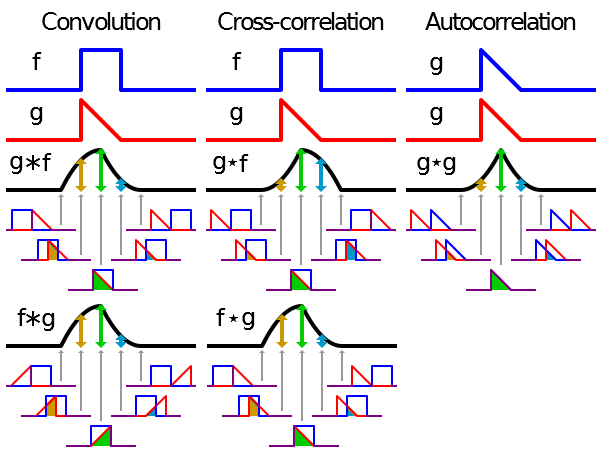
\includegraphics[width=0.6\textwidth]{figs/chp04/chp04_08_Comparison_convolution_james.pdf}
	\caption{卷积运算$g*f$,互相关运算$g \star f$和自相关运算$g \star g$示意图}
	\label{fig:chp04_08_Comparison_convolution_james}
\end{figure}

根据上述物理含义的差异,需要使用互相关运算来对输入图像和模板进行相似度度量。一般定义输入图像与滤波模板的互相关运算为
\begin{align}
g=h\text{ }\otimes  f  
\end{align}
其中$g$表示输出的响应图,$h$表示滤波模板,$f$表示输入图像,$\otimes$表示互相关运算。

由于互相关运算的时间消耗较大,因此需要使用快速傅里叶变换的方法进行转换。定义互相关函数的快速傅里叶变换,即计算费时的卷积运算转换为普通的点乘运算,
\begin{align}
\mathcal{F}(g) = \mathcal{F}(h\otimes f)={{\mathcal{F}(h)}^{*}}\odot \mathcal{F}(f )
\end{align}
其中,$\mathcal{F}$ 表示傅里叶变换,$\odot$ 表示每个元素的点乘,$h^*$ 表示函数 $h$ 的共轭。此时,时间计算开销为$O(n\log n)$,其中$n$是图像中像素的个数。

为了后续对H函数的求解过程的表达方便,将上式用新的符号标记为
\begin{align}
G=F\odot H^*
\end{align}
由于上式右侧的运算是对于每个元素的点乘,由此可以得到对$H^*$的解析解
\begin{align}
H^* = \frac{G}{F}
\end{align}

由于滤波器需要对跟踪目标区域周边$m$个区块进行搜索,因此设计的目标函数需要对每一个区域进行运算,并与实际输出进行对比。目标函数的数学表达为
\begin{align}
\underset{{{H}^{*}}}{\mathop{\min }}\,\sum\limits_{i=1}^{m}{|{{H}^{*}}\odot{{F}_{i}}-{{G}_{i}}{{|}^{2}}} 
\end{align}
即对每一个输入的图像$F_i$和实际输出$G_i$是在频域的运算结果,目标是寻找合适的滤波器$H$,使得该滤波器与输入图像进行互相关运算后的输出结果与实际输出结果之间的误差最小。在频率域中,每一个运算都作用在图像的每一个元素上,由此可得
\begin{align}
\underset{H_{w,v}^{*}}{\mathop{\min }}\,\sum\limits_{i=1}^{m}{|H_{w,v}^{*}{{F}_{w,v,i}}-{{G}_{w,v,i}}{{|}^{2}}} 
\end{align}
对目标函数求导,寻找解析解
\begin{align}
&\frac{\partial }{{\partial H_{w,v}^*}}\sum\limits_{i = 1}^m {(H_{w,v}^*{F_{w,v,i}} - {G_{w,v,i}}) \cdot } {(H_{w,v}^*{F_{w,v,i}} - {G_{w,v,i}})^{\rm{*}}}{\rm{ = }}0\\  &\Rightarrow \frac{\partial }{{\partial H_{w,v}^*}}\sum\limits_{i = 1}^m {H_{w,v}^*{F_{w,v,i}} \cdot {H_{w,v}}F_{w,v,i}^{\rm{*}} - H_{w,v}^*{F_{w,v,i}}G_{w,v,i}^{\rm{*}} - {H_{w,v}}F_{w,v,i}^{\rm{*}}G_{w,v,i}^{}{\rm{ + }}{G_{w,v,i}}G_{w,v,i}^{\rm{*}}} {\rm{ = }}0\\  
&\Rightarrow \sum\limits_{i = 1}^m {{F_{w,v,i}} \cdot {H_{w,v}}F_{w,v,i}^{\rm{*}} - {F_{w,v,i}}G_{w,v,i}^{\rm{*}}} {\rm{ = }}0\\  
&\Rightarrow {H_{w,v}}{\rm{ = }}\frac{{\sum\limits_{i = 1}^m {{F_{w,v,i}}G_{w,v,i}^{\rm{*}}} }}{{\sum\limits_{i = 1}^m {{F_{w,v,i}}F_{w,v,i}^{\rm{*}}} }}
\end{align}

根据上述求导公式,对区域中的每一个元素求解,可以得到函数最优解$H^*$的解析表达形式为
\begin{align}
H^*\text{=}\frac{\sum\limits_{i=1}^{m}{{{F}_{i}}\odot G_{i}^{\text{*}}}}{\sum\limits_{i=1}^{m}{{{F}_{i}}\odot F_{i}^{\text{*}}}} 
\end{align}

得到新的模板表达公示后,一般设计线性更新方式,得到对模板$H$的更新
\begin{align}
{{H}_{t}}=(1-\eta ){{H}_{t-1}}+\mu H(t) 
\end{align}
其中$\mu$是模板更新的学习速率。为化简更新公式,可以对分子和分母分别进行更新
\begin{align}
&H_t=\frac{A_t}{B_t}\\
&A_t=\mu F_t\odot G_t^*+(1-\mu)A_{t-1}\\
&B_t=\mu F_t\odot F_t^*+(1-\mu)B_{t-1}
\end{align}

在具体求解目标中心位置的过程中,通过将模板$H$与输入的图像$f$做相关运算,并在得到的响应图中,寻找数值最大的点,以此作为当前图像模板的所在位置。但由于MOOSE方法没有考虑模板尺寸的变化,因此无法适用于无人机由远及近过程中的跟踪问题。

 
\subsection{DDST方法} 
%Ref: http://blog.csdn.net/roamer_nuptgczx/article/details/50134633
%Ref: http://blog.csdn.net/autocyz/article/details/48651013
%Ref HOG: https://xiangjiang.live/2016/02/09/histograms-of-oriented-gradients/
%Discriminative Scale Space Tracking
针对MOOSE方法的缺陷,Discriminative Scale Space Tracking(DDST)方法通过设计两个不同的滤波器来解决该问题,其核心思想是利用多个维度的特征来分别描述目标的平移变换和尺度变换。

该方法主要设计两个滤波器来实现:
\begin{compactenum}
	\item 该方法设计平移变化滤波器来估计目标的平移变换情况,该滤波器计算每个像素点的一个一维灰度和和20维FHOG特征,最终计算出目标的最新位置。其中FHOG特征是指由Felzenszwalb提出的一种快速计算HOG特征的方法,该方法能够快速根据当前彩色图像计算出9个方向,32维的图像特征。为了提高后续处理的运算效率,这里只使用其中的前20个作为主要特征。
	\item 该方法设计一个尺度变化滤波器来估计目标的尺度变化情况,该滤波器将样本进行30种不同尺度的变换,通过提取上述每种变化中的20维FHOG特征,最终计算出目标的当前的尺寸变化。
\end{compactenum}



根据上述设计思路,一副图像可以使用$d$维特征来进行描述,定义在目标区域的一块图像的大小为$f$,对于不同维度的特征用$f^l,\ l \in {1, 2, ..., d}$来表达
\begin{align}
\underset{{{H}^{*}}}{\mathop{\min }}\,\sum\limits_{l=1}^{d}{|{{H}^{*}}\odot{{F}^{l}}-{{G}^{l}}{{|}^{2}}}+\lambda \sum_{l=1}^{d}|H^{l}|^2
\end{align}
其中等式右侧的第二项为正则项,主要用于避免在频域转换过程后,分母等于零的情况出现。对上式求微分,可以得到最优解的计算公式
\begin{align}
H^l\text{=}\frac{\sum\limits_{i=1}^{m}{{{F}^{l}}\odot {G^{i}}^{{*}}}}{\sum\limits_{i=1}^{d}{{{F}^{i}}\odot {F^{i}}^{\text{*}}}+\lambda}=\frac{A^{l}_{t}}{B^{l}_{t}+\lambda}
\end{align}
与MOOSE方法相同,分别对上述公式的分子和分母独立更新
\begin{align}
\label{eq:moose_at_update}
&A_t^l=(1-\mu)A_{t-1}^{l}+\mu G_{t}^{*}\odot F_{t}^{l}\\
&B_t^l=(1-\mu)B_{t-1}^{l}+\mu \sum_{l=1}^{d}{F_{t}^{l}}^{*}\odot F_{t}^{l}
\end{align}

在得到更新后的分子和分母后,在响应区域进行计算,并求解出目标位置
\begin{align}
\mathbf{y}_t=\mathcal{F}^{-1}(\frac{\sum_{i=1}^{d}{A^{l}_{t-1}}^*\odot Z^{l}_{t}}{B_{t-1}+\lambda})
\end{align}

平移部分计算的示意图如图\ref{fig:chp04_09_translation_map}所示。其中FHOG的基本运算可以参考文献\cite{lsvm-pami},对FHOG的C++与MATLAB代码实现可以参考\cite{voc-release5}。

\begin{figure}[ht]   
	\centering
	\includegraphics[width=\textwidth]{figs/chp04/chp04_09_translation_map.pdf}
	\caption{平移变化滤波器}
	\label{fig:chp04_09_translation_map}
\end{figure}

对于尺度变化滤波器对图像进行变换的选择,通常采用如下方法。定义当前目标的尺度为$P\times R$,则定义$a = 1.05$作为横向尺度因子,$b = 1.02$作为纵向尺度因子,$S=30$作为尺度滤波器的宽度,则序列尺寸的变化可以通过如下公式计算得到
\begin{align}
a^nP_{t-1}\times b^nR_{t-1}\ ,n \in \{-\frac{S-1}{2},...,\frac{S-1}{2}\} 
\end{align}
上述$a$和$b$两个因子的选择主要是依赖无人机的原始尺寸。尺度变换部分计算的示意图如图\ref{fig:chp04_10_scale_map}所示。
\begin{figure}[ht]   
	\centering
	\includegraphics[width=\textwidth]{figs/chp04/chp04_10_scale_map.pdf}
	\caption{尺度变化滤波器}
	\label{fig:chp04_10_scale_map}
\end{figure}
对于多尺度问题,通过在目标区域提取$M\times N \times S$的立方体,其中$M$和$N$代表高和宽,$S$代表尺度等级,构造一个三维高斯函数,并计算互相关输出。这种方法实际就是把上述两个滤波器结合起来,构成一个新的三维空间滤波器进行滤波。


为了更快的运行上述算法,可以使用Sub-gird迭代方法进行优化。该方法是信号领域的一种迭代方法\cite{oppenheim1996signals}。Sub-grid迭代求解互相关值
\begin{align}
\mathbf{y}_t=\mathcal{F}^{-1}(\frac{\sum_{i=1}^{d}{A^{l}_{t-1}}^*\odot Z^{l}_{t}}{B_{t-1}+\lambda})
\end{align}
其中在$Y_t$的高频位置采用Zero-Padding方法来进行优化提速。

此外,DSST计算的时间开销主要是FFT运算,因此可以通过使用采样维度下降的方法进行进一步优化, 跟踪目标模板$u_t$的更新不再使用线性更新方法
\begin{align}
u_t = (1-\mu)u_{t-1}+\mu f_t
\end{align}
根据傅里叶变换的线性化特点,公式\ref{eq:moose_at_update}中$A_t^l$的求解公式可以化简为
\begin{align}
A_t^l=G^* \mathcal{F}(u_t^l)
\end{align}
由此,对模板$u_t$的更新转换为,建立一个映射矩阵$P_t$,其维度大小是$\hat{d} \times d$,其中$\hat{d}$是压缩特征的维数。

该矩阵的计算方式通过使构造误差最小得到,即最小化公式
\begin{align}
\epsilon=\sum_\mathbf{n}||u_t(\mathbf{n})-P_t^TP_tu_t(\mathbf{n})||^2
\end{align}
其中$\mathbf{n}$是在模板$u_t$中的一个元素。当映射矩阵满足$P_tP_t^T=I$时得到最优解,具体求解方式是对Auto-Correlation矩阵进行特征值分解
\begin{align}
C_t=\sum_{\mathbf{n}}u_t(\mathbf{n})u_t(\mathbf{n})^T
\end{align}
其中映射矩阵$P_t$的每一行是$C_t$矩阵的特征向量。

所以,分子和分母的更新方法转换为
\begin{align}
&\hat{A}_t^l=G^*\hat{U}_t\\
&\hat{B}_t^l=(1-\mu) \hat{B}_{t-1}^{l}+\mu \sum_{l=1}^{\hat{d}}\hat{F}_t^{l*}\hat{F}^l_t
\end{align}
其中
\begin{align}
\hat{F}_t=\mathcal{F}(P_tf_t)\\
\hat{U}_t=\mathcal{F}(P_tu_t)
\end{align}

使用压缩后的采样后,响应函数的输出变换为
\begin{equation}
\mathbf{y}_t={\mathcal{F}^{-1}}(\frac{\sum_{i=1}^{\hat{d}}{\hat{A}^{*l}_{t-1}} \odot \hat{Z}^{l}_{t}}{\hat{B}_{t-1}+\lambda})
\end{equation}

为了测试DSST方法,选用小型无人机和中型无人机的两类数据集共七组进行测试。其中DSST方法中的参数除了上述定义之外,实验中使用的目标函数正则化参数$\lambda=0.01$, 学习速率$\mu=0.025$。图\ref{fig:chp04_11_small_uav_cle}和\ref{fig:chp04_12_small_uav_overlap}所示为小型无人机数据集的第一组结果。图\ref{fig:chp04_13_middle_uav_cle}和\ref{fig:chp04_14_middle_uav_overlap}所示为中型无人机数据集的第一组结果。对于小型无人机的结果可以发现,在长度为350帧的目标跟踪过程中,中心点出现过两次较大偏差,其主要原因是在相应的两帧,转台出现了抖动(通过查询响应帧的转台返回数据)。从整体情况来看,在小型无人机的纵向跟踪误差略大于横向误差,其主要原因是转台在俯仰方向的运动相对较大。
\begin{figure}[ht]   
	\centering
	\includegraphics[width=0.8\textwidth]{figs/chp04/chp04_11_small_uav_cle.pdf}
	\caption{小型无人机第一组数据中心点偏差情况}
	\label{fig:chp04_11_small_uav_cle}
\end{figure}

\begin{figure}[ht]   
	\centering
	\includegraphics[width=0.8\textwidth]{figs/chp04/chp04_12_small_uav_overlap.pdf}
	\caption{小型无人机第一组数据矩形框覆盖率情况}
	\label{fig:chp04_12_small_uav_overlap}
\end{figure}

\begin{figure}[ht]   
	\centering
	\includegraphics[width=0.8\textwidth]{figs/chp04/chp04_13_middle_uav_cle.pdf}
	\caption{中型无人机第一组数据中心点偏差情况}
	\label{fig:chp04_13_middle_uav_cle}
\end{figure}

\begin{figure}[ht]   
	\centering
	\includegraphics[width=0.8\textwidth]{figs/chp04/chp04_14_middle_uav_overlap.pdf}
	\caption{中型无人机第一组数据矩形框覆盖率情况}
	\label{fig:chp04_14_middle_uav_overlap}
\end{figure}

使用DSST方法在七组不同数据集的测试结果如表\ref{lab:dsst_seven_results}所示,其中平均中心偏差的结果和误差带如图\ref{fig:chp04_15_seven_cle}所示,图\ref{fig:chp04_16_seven_speed}描述了无人机在七组不同数据集的跟踪速率。通过比较中型无人机和小型无人机可以得到以下结论:
\begin{compactenum}
	\item 小型无人机的中心点误差小于中型无人机。其主要原因是小型无人机的成像面积较小,在近端成像时,机头中心位置的成像最为明显。而中型无人机由于成像面积大,机身的整体图像信息对中心点的影响相对较大。
	\item DSST方法的解算精读鲁棒性较强。实验中两种类型的数据集使用相同的DSST参数,七组数据的中心点误差均控制在5个像素以下。	
	\item DSST方法的速度严重受制于目标图像尺寸。
\end{compactenum}

\begin{table}[ht]
	\centering
	\caption{DSST方法在七组不同数据集的测试结果}
	\label{lab:dsst_seven_results}
	\begin{tabular}{lcccc}
		\hline
		& \begin{tabular}[c]{@{}c@{}}Center Location \\ Error(Pixel)\end{tabular} & \begin{tabular}[c]{@{}c@{}}Distance \\ Precision (\%)\end{tabular} & \begin{tabular}[c]{@{}c@{}}Overlap \\ Precision(\%)\end{tabular} & Speed (fps) \\ \hline
		\multicolumn{1}{c}{小型尺寸无人机第一组} & 3.41                                                                    & 97.53                                                              & 74.32                                                            & 32.31       \\
		\multicolumn{1}{c}{小型尺寸无人机第二组} & 3.27                                                                    & 98.12                                                              & 75.23                                                            & 30.13       \\
		小型尺寸无人机第三组                     & 3.12                                                                    & 98.23                                                              & 74.34                                                            & 29.12       \\
		小型尺寸无人机第四组                     & 2.80                                                                    & 96.84                                                              & 74.32                                                            & 31.84       \\ \hline
		中型尺寸无人机第一组                     & 4.67                                                                    & 94.94                                                              & 85.35                                                            & 10.65       \\
		中型尺寸无人机第二组                     & 4.93                                                                    & 95.14                                                              & 83.35                                                            & 12.31       \\
		中型尺寸无人机第三组                     & 4.12                                                                    & 95.31                                                              & 82.66                                                            & 11.98       \\ \hline
	\end{tabular}
\end{table}
\begin{figure}[ht]   
	\centering
	\includegraphics[width=0.8\textwidth]{figs/chp04/chp04_15_seven_cle.pdf}
	\caption{七组数据集平均中心偏差结果}
	\label{fig:chp04_15_seven_cle}
\end{figure}

\begin{figure}[ht]   
	\centering
	\includegraphics[width=0.8\textwidth]{figs/chp04/chp04_16_seven_speed.pdf}
	\caption{七组数据集平均运算帧频结果}
	\label{fig:chp04_16_seven_speed}
\end{figure}


\section{引入转台运动后的目标位置估计}
\subsection{低通滤波器的设计}
无人机的目标在像平面的投影通常是由多个像素点组成,上述目标识别算法主要通过求解所有像素点的几何平均位置来作为后续转台控制和无人机位置解算的输入。由于相机在成像过程中存在噪声扰动,所以图像识别之后的结果也会受到噪声的污染,因此本节设计一个低通滤波器对目标的位置和移动速度进行滤波。

一般情况,均认为系统的图像采样时间间隔基本相同。但通过实际测试实验发现系统采样时间抖动较大,其中一组降落过程中的图像采样时间间隔情况如图\ref{fig:chp04_01_delta_time_stamp}所示。图中的蓝色实线表明系统在最后18\ s左右的降落过程中,系统的采样出现较大的波动,其峰值甚至达到190\ ms。所以,在进行像平面位置估计等计算时,需要实时计算每一帧的采样时间间隔,以此来提升解算精度。

\begin{figure}[ht]   
	\centering
	\includegraphics[width=0.8\textwidth]{figs/chp04/chp04_01_delta_time_stamp.pdf}
	\caption{一组降落实验中的图像时间间隔采样情况}
	\label{fig:chp04_01_delta_time_stamp}
\end{figure}

定义目标的在像平面的坐标为$\mathbf{p}_{uav} = (u, v)^T$,经过低通滤波器之后的像平面坐标为$\bar{\mathbf{p}}_{uav} = (\bar{u}, \bar{v})^T$,目标点的移动速度定义为$\dot{\mathbf{p}}_{uav} = (\dot{u},\dot{v})^T$。根据低通滤波器的定义,可以得到目标原始位置坐标和滤波之后坐标之间的关系
\begin{align}
\mathbf{p}(s) = \frac{1}{\tau s+1}\bar{\mathbf{p}}
\end{align}
对上式微分可以得到速度与滤波之后坐标之间的关系
\begin{align}
\dot{\mathbf{p}}(s) = \frac{s}{\tau s+1}\bar{\mathbf{p}}
\end{align}
由于采样是离散系统,因此将上式进行双线性变换(Bilinear Transform)\cite{franklin1998digital},即将连续系统转换离散系统,通过下式进行变换
\begin{align}
s \mapsto \frac{2}{T_s}\frac{z-1}{z+1}
\end{align}
带入后可以得到
\begin{align}
\mathbf{p}[z] &= \frac{1}{\frac{2}{T_s}\frac{z-1}{z+1}}\bar{\mathbf{p}} \\
&= \frac{\frac{T_s}{2\tau+T_s}(z+1)}{z-\frac{2\tau-T_s}{2\tau+T_s}}\bar{\mathbf{p}}
\end{align}
和
\begin{align}
\dot{\mathbf{p}}[z] &= \frac{\frac{2}{T_s}\frac{z-1}{z+1}}{\frac{2}{T_s}\frac{z-1}{z+1}+1}\bar{\mathbf{p}} \\
&= \frac{\frac{2}{2\tau+T_s}(z-1)}{z-\frac{2\tau-T_s}{2\tau+T_s}}\bar{\mathbf{p}}
\end{align}
对上式两个公式进行逆z变换,可以得到求解期望位置的差分公式
\begin{align}
\mathbf{p}[n] = \frac{2\tau-T_s}{2\tau+T_s} \mathbf{p}[n-1]+ \frac{T_s}{2\tau+T_s}(\bar{\mathbf{p}}[n-1] + \bar{\mathbf{p}}[n-1] )
\end{align}
同理得到求解期望速度的差分公式为
\begin{align}
\dot{\mathbf{p}}[n] = \frac{2\tau-T_s}{2\tau+T_s}\dot{\mathbf{p}}[n-1]+ \frac{2}{2\tau+T_s}(\bar{\mathbf{p}}[n-1] - \bar{\mathbf{p}}[n-1] )
\end{align}
其中$\mathbf{p}[0] = \bar{\mathbf{p}}[0]$和$\dot{\mathbf{p}}[0] = 0$,$\tau$是滤波的阶段频率,$T_s$是每次采样时间间隔。


\subsection{引入转台信息后的位置估计}
由于受到采样间隔时间和转台系统误差的影响,转台在俯仰角和方位角的返回值同样存在较大偏差。左右两侧转台在一组降落过程中的末状态角度读取结果和偏差计算如图\ref{fig:chp04_02_pan_tilt_status}所示。其中,图中的蓝色虚线为通过串口读取到的转台实际角度,橙色实线为相邻两次采样之间转台的变化量。通过曲线的趋势可以看到,由于采样时间的波动,转台俯仰角和方位角的变化率整体平稳,在$12\ s$到$16\ s$之间,两个转台的俯仰角和横滚角都出现了较大的几次波动,这几次波动与图\ref{fig:chp04_01_delta_time_stamp}响应时刻的采样间隔变大相吻合。同时,突然出现的较大延时,还会对转台控制系统和目标在位置中的估计带来较大影响,因此不能仅仅依赖目标在图像中的位置来中下一帧的位置进行估计,而是需要通过读取转台的角度信息来对原有模型进行修正。
\begin{figure}[ht]   
	\centering
	\includegraphics[width=\textwidth]{figs/chp04/chp04_02_pan_tilt_status.pdf}
	\caption{时间采样间隔的对转台读数的影响情况}
	\label{fig:chp04_02_pan_tilt_status}
\end{figure}

在转台转动情况已知的情况下,如果目标相对于引导坐标系不动,则可以得到其在像平面的运动情况。定义$P_c$是目标点在相机坐标系的一点,$P_r$是目标点在引导坐标系的一点,两个坐标系之间的转换关系为
\begin{equation}
P_r = T_c P_c
\end{equation}
其中$T_c$是一个$4 \times 4$转换矩阵,将相机坐标系的一点转换为引导坐标系的一点。考虑到转台的转动情况定义当前时刻转换矩阵为$T_c(t)$,在相机坐标系的坐标为$P_c(t)$ 上一时刻的转换矩阵为$T_c(t-1)$,在相机坐标系的坐标为$P_c(t-1)$。在目标点相对于引导坐标系不变的情况下,该点的坐标系可以表示为
\begin{equation}
P_r = T_c(t) P_c(t) =T_c(t-1) P_c(t-1)
\end{equation}

通过变换可以得到
\begin{equation}
\label{eq:chp04_predict_position}
P_c(t-1) = T_c(t-1)^{-1}T_c(t) P_c(t)
\end{equation}

由于转台的读数可以获得,因此转换矩阵之间的关系可以表示为

\begin{equation}
T_c(t) = R_Y(\psi)R_X(\phi)T_c(t-1)
\end{equation}

同理可得
\begin{equation}
T_c(t-1)^{-1} = T_c(t)^{-1}R_Y(\psi)R_X(\phi)
\end{equation}

带入\ref{eq:chp04_predict_position}式之后,可以得到
\begin{equation}
P_c(t-1) =T_c(t)^{-1}R_Y(\psi)R_X(\phi)T_c(t) P_c(t)
\end{equation}

因为实验所用转台的最小转动角度为$0.006 \degree$,可以将转换矩阵的相关量进行近似求解
\begin{align}
&\cos \phi \approx \cos \psi \approx 1 \\
&\sin \phi \approx \phi \\
&\cos \psi \approx \psi \\
&\sin \phi \approx \sin \psi \approx 0 \\
\end{align}

如果初始状态,系统存在水平方向的偏差角度$\theta$,则此时的转换矩阵为
\begin{equation}
T_c(t) =\begin{pmatrix} 1 & 0 & 0 & 0 \\ 0 & \cos \theta & -\sin \theta & \rho_y \\0 & \sin \theta & \cos \theta & \rho_z \\ 0 & 0 & 0 &0 \end{pmatrix}
\end{equation}

\begin{equation}
T_c(t)^{-1} =\begin{pmatrix} 1 & 0 & 0 & 0 \\ 0 & \cos \theta & \sin \theta & -\cos \theta \rho_y -\sin \theta \rho_z \\0 & -\sin \theta & \cos \theta & \sin\theta \rho_y-\cos \theta \rho_z \\ 0 & 0 & 0 & 1 \end{pmatrix}
\end{equation}
带入上述公式之后,可以得到
\begin{align}
&X_{t-1} = X_t + \psi \sin \theta Y_t + \psi \cos \theta Z_t + \psi \rho_z \\
&Y_{t-1} = -\psi \sin \theta X_t +  Y_ t - \phi Z_t + \phi \sin \theta \rho_y - \phi \cos \theta \rho_z \\
&Z_{t-1}  = -\psi \cos \theta X_t + \phi  Y_ t + Z_t + \phi \cos \theta \rho_y - \phi \sin \theta \rho_z
\end{align}
根据相机的针孔成像模型
\begin{equation}
x = f \frac{X}{Z}
\end{equation}
则像素的向后递推公式为
\begin{align}
x_{t-1} = f\frac{x_t+\psi \sin \theta y_t + f\psi \cos \theta}{- \psi \cos \theta x_t + \phi y_t + f} \\
y_{t-1} = f\frac{-\psi \sin \theta x_t +y_t -f\phi}{- \psi \cos \theta x_t + \phi y_t + f} \\
\end{align}
当系统的初始偏差不存在时,向后地推公式可以表达为
\begin{align}
\label{eq:curr_predict_prev]}
x_{t-1} = f\frac{x_t + f\psi }{- \psi  x_t  + \phi y_t + f} \\
y_{t-1} = f\frac{y_t -f\phi}{- \psi  x_t + \phi y_t + f}
\end{align}
同理,如果已知上一帧位置和转台转动的情况,可以推算出当前帧的像素位置
\begin{align}
\label{eq:prev_predict_curr}
x_{t} = f\frac{x_{t-1} - f\psi }{x_{t-1}  \psi  - \phi y_{t-1} + f} \\
y_{t} = f\frac{y_{t-1} -f\phi}{  x_{t-1} \psi - \phi y_{t-1} + f} \\
\end{align}

根据上述方法定义,在实际数据中可以得到进一步验证。图\ref{fig:chp04_17_predict_1}和图\ref{fig:chp04_18_predict_2}所示为选取两组转台方位角和俯仰角偏差较大的情况。其中上一帧目标坐标位置的真值用黄色点标记,根据上一帧坐标预测出的当前帧坐标用蓝色点标记。此外,当前帧坐标真值用绿色标记,通过当前帧真值反向预测上一帧目标位置的坐标用墨绿色标记。通过比较向前和向后预测的真值,可以验证之前的推算是正确。

图\ref{fig:chp04_17_predict_1}左侧是中心无人机第一组降落数据集中第138帧的数据,右侧为第139帧的数据,通过直观比较左右两幅图像的地平线位置,并参考转台提供的数据可以判断出:转台在连续两帧中俯仰角的变化较大。同理,图\ref{fig:chp04_17_predict_1}所示是该组图像序列的第104帧和第105帧图像,通过比较两幅图像白色文字右侧的地面栏杆变化,并参考转台提供的数据可以判断出:转台在连续两帧中方位角变化较大。通过公式\ref{eq:prev_predict_curr}可以对该部分偏差进行有效修正,同时也可以通过公式\ref{eq:prev_predict_curr}来反向验证算法是否有效。这两组图像的具体数据结果如表所示。

\begin{figure}[ht]
	\centering
	\includegraphics[width=\textwidth]{figs/chp04/chp04_17_predict_1.pdf}
	\caption{当转台出现方位角较大偏差时,目标位置的估计情况}
	\label{fig:chp04_17_predict_1}
\end{figure}

\begin{figure}[ht]   
	\centering
	\includegraphics[width=\textwidth]{figs/chp04/chp04_18_predict_2.pdf}
	\caption{当转台出现俯仰角较大偏差时,目标位置的估计情况}
	\label{fig:chp04_18_predict_2}
\end{figure}

\begin{table}[]
	\centering
	\caption{引入转台信息后的位置估计结果}
	\label{my-label}
	\begin{tabular}{lccc|ccc}
		\hline
		& \multicolumn{3}{c|}{x方向坐标(pixel)}                         & \multicolumn{3}{c}{y方向坐标(pixel)}   \\ \cline{2-7} 
		& 真实值 & \multicolumn{1}{l}{估计值} & \multicolumn{1}{l|}{误差值} & 真实值 & 估计值 & \multicolumn{1}{l}{误差值} \\ \hline
		\multicolumn{1}{c}{第104帧} & 287 & 299                     & -12                      & 271 & 270 & 1                       \\
		\multicolumn{1}{c}{第105帧} & 307 & 295                     & 12                       & 267 & 268 & -1                      \\ \hline
		第138帧                     & 450 & 464                     & -14                      & 329 & 308 & 21                      \\
		第139帧                     & 444 & 430                     & 14                       & 284 & 304 & -20                     \\ \hline
	\end{tabular}
\end{table}

\section{本章小结}
本章首先将无人机降落过程中的目标跟踪问题划归为One-shot Tracking问题,即通过目标识别方法或人工选取来得到跟踪目标的初始位置。其次,根据无人机降落过程中的成像特性,选用形态学滤波方法对左右视觉传感器采集到的图像进行预处理。随后,通过改进TLD方法、主动轮廓线方法和相关滤波三种方法,来尽可能的实现对无人机目标的实时跟踪和中心点位置估计。最后,通过引入转台的方位角和俯仰角信息对无人机目标的位置进行进一步修正,并基于修正后的位置使用上述三种目标识别方法,最终能够提升对中心点位置估计的稳定性和可靠性,系统的整体工作示意图如图\ref{fig:chp04_19_tracking_diagram}所示。


\begin{figure}[ht]   
	\centering
	\includegraphics[width=\textwidth]{figs/chp04/chp04_19_tracking_diagram.pdf}
	\caption{当转台出现俯仰角较大偏差时,目标位置的估计情况}
	\label{fig:chp04_19_tracking_diagram}
\end{figure}
